%\subsection{Schema generale: definizione di un alert con estensioni}
%\begin{figure}[H]
%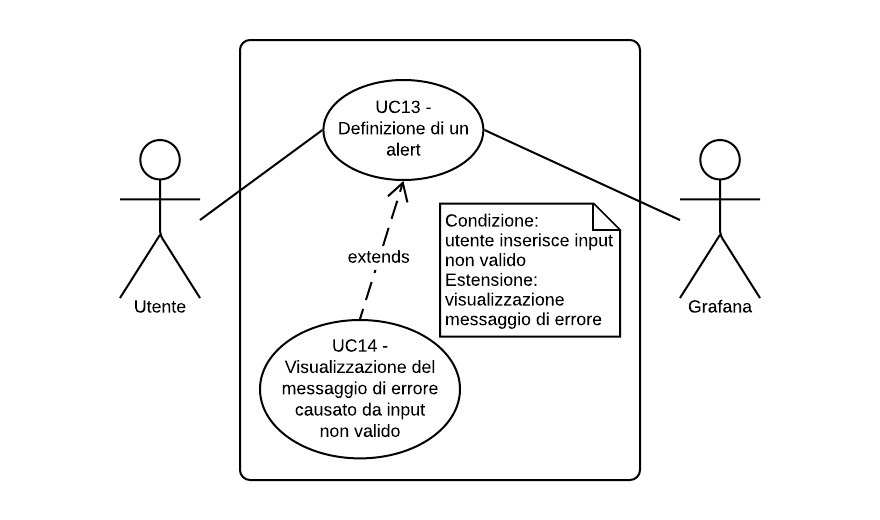
\includegraphics{img/UC13 - Schema generale.png}
%\caption{Schema generale: definizione di un alert con estensioni}
%\end{figure}
\subsection{UC13 - Definizione di un alert}
\begin{figure}[H]
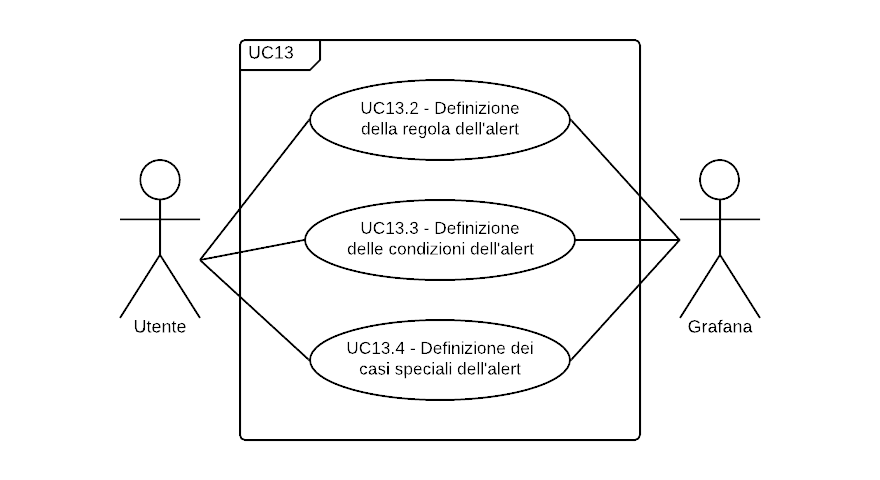
\includegraphics{img/UC13_-_Definizione_di_un_alert.png}
\caption{Diagramma degli use case di UC13}
\end{figure}
\begin{itemize}
	\item \textbf{Codice identificativo}: UC13;
	\item \textbf{Titolo}: definizione di un alert\glo;
	\item \textbf{Attore primario}: utente;
	\item \textbf{Attore secondario}: Grafana\glo;
	\item \textbf{Descrizione}: questo caso d'uso\glosp descrive la funzionalità, offerta da Grafana\glo, di definire alert\glosp sui dati che vengono monitorati;
	\item \textbf{Precondizione}: l'utente è autenticato nel sistema software Grafana\glosp ed è presente una istanza di Grafana\glosp cloud o locale su cui è stato aggiunto un pannello grafico che monitora una serie di dati;
	\item \textbf{Postcondizione}: viene inserito e definito con successo un alert\glosp nel pannello grafico scelto;
	\item \textbf{Scenario principale}: 
	\begin{enumerate}
		\item definizione della regola dell'alert\glosp (UC13.2);
		\item definizione delle condizioni dell'alert\glosp (UC13.3);
		\item definizione dei casi speciali dell'alert\glosp (UC13.4).
	\end{enumerate}

	\item \textbf{Estensioni}:	
	\begin{enumerate}
		\item visualizzazione del messaggio di errore causato da input non valido (UC13).
	\end{enumerate}
\end{itemize}

\subsubsection{UC13.2 - Definizione della regola di un alert}
\begin{itemize}
	\item \textbf{Codice identificativo}: UC13.2;
	\item \textbf{Titolo}: definizione della regola dell'alert\glo;
	\item \textbf{Attore primario}: utente;
	\item \textbf{Attore secondario}: Grafana\glo;
	\item \textbf{Descrizione}: dopo aver aggiunto un alert\glosp ad un pannello grafico l'utente ha la possibilità di definire la regola principale di funzionamento dell'alert\glosp che comprende: la scelta del nome, un valore che indica l'intervallo di tempo tra i controlli sui dati e un valore che indica per quanto tempo continuare il controllo;
	\item \textbf{Precondizione}: l'utente ha aggiunto un alert\glosp al pannello grafico;
	\item \textbf{Postcondizione}: l'utente tramite le funzioni offerte da Grafana\glosp ha definito la regola dell'alert\glosp precedentemente aggiunto;
	\item \textbf{Scenario principale}: l'utente definisce le regole di funzionamento dell'alert\glosp appena inserito, usando le funzioni previste da Grafana\glosp ed inserendo nome e tempi di interrogazione.
\end{itemize}

\subsubsection{UC13.3 - Definizione delle condizioni di un alert}
\begin{itemize}
	\item \textbf{Codice identificativo}: UC13.3;
	\item \textbf{Titolo}: definizione delle condizioni dell'alert\glo;
	\item \textbf{Attore primario}: utente;
	\item \textbf{Attore secondario}: Grafana\glo;
	\item \textbf{Descrizione}: dopo aver aggiunto un alert\glosp ad un pannello grafico l'utente ha la possibilità di definire le sue condizioni di funzionamento, cioè i limiti che, se superati, portano alla visualizzazione dei dati oltre la soglia prestabilita, nel pannello grafico;
	\item \textbf{Precondizione}: l'utente ha aggiunto un alert\glosp al pannello grafico;
	\item \textbf{Postcondizione}: l'utente tramite le funzioni offerte da Grafana\glosp ha definito una o più condizioni dell'alert\glosp precedentemente aggiunto;
	\item \textbf{Scenario principale}: l'utente definisce le condizioni di funzionamento dell'alert\glosp appena inserito, usando le funzioni previste da Grafana\glosp e selezionando la funzione di aggregazione dati ed il valore soglia che attiva l'allarme.
\end{itemize}

\subsubsection{UC13.4 - Definizione dei casi speciali di un alert}
	\begin{itemize}
	\item \textbf{Codice identificativo}: UC13.4;
	\item \textbf{Titolo}: definizione dei casi speciali dell'alert\glo;
	\item \textbf{Attore primario}: utente;
	\item \textbf{Attore secondario}: Grafana\glo;
	\item \textbf{Descrizione}: dopo aver aggiunto un alert\glosp ad un pannello grafico l'utente ha la possibilità di definire il suo comportamento al verificarsi di casi particolari, come nel caso in cui non ci sono dati o sono tutti nulli, oppure nel caso in cui la richiesta va in timeout o c'è un errore di esecuzione;
	\item \textbf{Precondizione}: l'utente ha aggiunto un alert\glosp al pannello grafico;
	\item \textbf{Postcondizione}: l'utente, tramite le funzioni offerte da Grafana\glosp, ha definito uno o più comportamenti speciali dell'alert\glosp precedentemente aggiunto;
	\item \textbf{Scenario principale}: l'utente definisce i comportamenti speciali dell'alert\glosp nei casi particolari come assenza di dati o errori di esecuzione. Per farlo utilizza le funzioni previste da Grafana\glosp selezionando i comportamenti desiderati.
\end{itemize} 
